\chapter{System Maintenance}

\section{Environment}

\subsection{Software}
Throughout the development of my program, I have used a wide variety of different programs
\begin{itemize}
    \item Python 3.4.1
    \item Python's IDLE (Integrated DeveLopment Environment)
    \item PyQt 4
    \item SQLite3
    \item SQLite Inspector
    \item Mozilla Firefox
\end{itemize}


\subsection{Usage Explanation}

\begin{center}
    \begin{tabular}{|p{3cm}|p{8cm}|}
	\hline
	\textbf{Software} & \textbf{Explanation} \\ \hline
	{Python 3.4.1} & {Python is my most proficient 4th generation language to create with. It is the most ideal programming language I know currently for the problems I wanted to solve. Version 3.4.1 is also ideal as some very useful modules only work with this version type.} \\ \hline
	{Python's IDLE} & {This was used for typing out the code. It provides very useful code-coloring for syntax so its simple to see if you've made certain errors before compiling. It also gives options for character editing so you can make it easier to see your code and in a preferred font.} \\ \hline
	{PyQt 4} & {This is the GUI module I'm using to create the visual part of the software. It works well to achieve the kind of visual look and abilities I want in my program.} \\ \hline
	{SQLite3} & {This is the database module I'm using to create and manage the database part of the program. It allows me to use SQL to manage database files from Python, meaning it can be inbuilt into the program.} \\ \hline
	{SQLite Inspector} & {A database viewing software. This was used for seeing if my Python code was successful in interacting with a database and testing SQL statements before adding them to my program.} \\ \hline
	{Mozilla Firefox} & {A web browser I used to download the various programs and modules needed in the creation of my software, as well as letting solve issues with my program by searching the issue on line.} \\ \hline

    \end{tabular}
\end{center}

\section{System Overview}

%use as many subsections as necessary for the system components
\subsection{System Component}

\section{Code Structure}

%use as many subsections as necessary for the code sections
\subsection{Particular Code Section}
%the code below can be uncommented and used to get a code section from a particular file
\begin{comment}
\begin{figure}[H]
    \pythonfile[firstline=5,lastline=10]{./tex/function_programs/print_function.py}
    \caption{The print() function} \label{fig:print_function}
\end{figure}
\end{comment}

\section{Variable Listing}

\section{System Evidence}

\subsection{User Interface}

\subsection{ER Diagram}
\begin{figure}[H]
    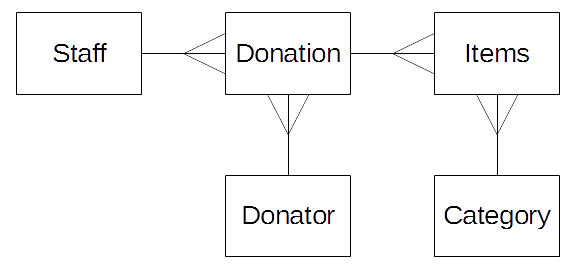
\includegraphics[width=\textwidth]{./Maintenance/Images/ERDiagram.png}
\end{figure}

\subsection{Database Table Views}

\subsection{Database SQL}

\subsection{SQL Queries}

\section{Testing}

My test results show that a clear indication of an incomplete project. The vast majority of the planned functionality is missing, even to go as far as a lack of interaction with a database file. Admittedly, due to the lack of functionality in the program, it did make the testing section rather easy to fill out. I guess for a solution to my issues would be to complete more of the functionality of the program, even if it was buggy or unstable. The testing also revealed that the select pieces of functionality that my program does have is very limited and does not include some of the aspects they should (a glaring example would be the lack of validation when inputting data).
\subsection{Summary of Results}

\subsection{Known Issues}
\begin{itemize}
    \item Missing Administative features
    \item Missing Administrator menu
    \item Missing Login menu
    \item Missing Password system
    \item Missing Change user feature
    \item Missing Add Donation feature
    \item Missing 
    \item Missing 
    \item Missing 
    \item Missing 
    \item Missing 
    \item Missing 
    \item Missing 
    \item Missing 
    \item Missing 


\end{itemize}

\section{Code Explanations}

\subsection{Difficult Sections}

\subsection{Self-created Algorithms}
\begin{python}
def Query (sql, data, multiBinds, method):
    with sqlite3.connect("charityShop.db") as db:
        cursor = db.cursor()
        cursor.execute("PRAGMA foreign_keys = ON")
        if not multiBinds:
            cursor.execute(sql, (data,))
        else:
            cursor.execute(sql, data)
        if method == "Select":
            selected = cursor.fetchone()
            db.commit()
            return(selected)
        db.commit()



def EntSelect():
    print("Would you like to change...")
    print()
    print("1. Staff")
    print("2. Donator")
    print("3. Category")
    print("4. Item")
    print("5. Donation")
    print("6. Return to previous menu")
    print()
    selection = int(input(">>"))
    print()
    if selection == 1:
        Questioned, ListedFields = SelectStaff()
        return(Questioned, ListedFields)
    elif selection == 2:
        Questioned, ListedFields = SelectDonator()
        return(Questioned, ListedFields)
    elif selection == 3:
        Questioned, ListedFields = SelectCategory()
        return(Questioned, ListedFields)
    elif selection == 4:
        Questioned, ListedFields = SelectItem()
        return(Questioned, ListedFields)
    elif selection == 5:
        Questioned, ListedFields = SelectDonation()
        return(Questioned, ListedFields)
    else:
        return (0,0)

def Insert():
    with sqlite3.connect("charityShop.db") as db:
        Questioned, ListedFields = EntSelect()
        if Questioned == 0:
            return(0)
        cursor = db.cursor()
# Since the format of the string is very specfic, it would require it to be hardcoded from every seperate entity and every action
# Instead, I have made it so that it manipulates the contents of the ListFields list (which contains the names for every part of every entity)
# The string is therefore constucted by using FOR loops and string editing, so this process can be applied to whatever I throw at it
        completeList = (ListedFields[0] + " (" + ListedFields[1])
        for count in range(len(ListedFields)-2):
            completeList = (completeList + ", " + ListedFields[count+2])    
        completeList = (completeList + ")")
        sql = "insert into {} values {}".format(completeList, Questioned)
        values = []
        for count in range(len(ListedFields) - 1):
            values.append(0)
        for count in range(len(ListedFields) - 1):
            values[count] = input("Enter the {} :".format(ListedFields[count +1]))
        values = tuple(values)
        Query(sql, values, True, "Insert")
        completion = 1
        return(1)

def SelectStaff():
    Questioned = "(?,?,?)"
    ListedFields = ["Staff", "StaffID", "StaffFirstName", "StaffLastName"]
    return(Questioned, ListedFields)

def SelectDonator():
    Questioned = "(?,?,?,?,?,?,?,?,?)"
    ListedFields = ["Donator", "DonatorID", "DonatorFirstName", "DonatorLastName", "DonatorAddress1", "DonatorAddress2", "DonatorCity", "DonatorCounty", "DonatorPostCode", "DonatorContact"]
    return(Questioned, ListedFields)

def SelectCategory():
    Questioned = "(?,?)"
    ListedFields = ["Category", "ItemCategory", "ItemCategoryDescription"]
    return(Questioned, ListedFields)

def SelectItem():
    Questioned = "(?,?,?,?,?,?)"
    ListedFields = ["Item", "ItemCode", "ItemDescription", "ItemPrice", "ItemCategory", "ItemQualityCheck", "ItemStatus"]
    return(Questioned, ListedFields)

def SelectDonation():
    Questioned = "(?,?,?,?,?)"
    ListedFields = ["Donation", "DonationCode", "ItemCode", "DonatorID", "StaffID", "Date"]
    return(Questioned, ListedFields)
\end{python}
\section{Settings}

\section{Acknowledgements}
I have not used or modified any code created by another person in my project.
\section{Code Listing}
\begin{landscape}
%include as many subsections as you have modules
\subsection{Module 1}
%the code below can be uncommented and used to get a code section from a particular file
\begin{comment}
\pythonfile[firstline=5]{./tex/function_programs/print_function.py}
\end{comment}
\end{landscape}
